\setchapterpreamble[ur][.6\textwidth]{%
\dictum[Fyodor Dostoyevsky, \textit{The Idiot} (1868--9)]{%
One can't understand everything at once, we can't begin with perfection all at once! In order to reach perfection one must begin by being ignorant of a great deal. And if we understand things too quickly, perhaps we shan't understand them thoroughly.}\vskip1em

\dictum[dude]{%
things}\vskip1em}

\chapter[Chapter 1: General introduction]{General introduction}
\chaptermark{General introduction}
%%%%%%%%%%%%%%%%%%%%%%%%%%%%%%%%%%%%%%%%%%%%%%%%%%%%%%%%%%%%%%%%%%%%%%%%%%%%%%%%%%%%%%

%%%%%%%%%%%%%%%%%%%%%%%%%%%%%%%%%%%%%%%%%%%
\section{Variation in fitness}
%variation in evolution
Understanding variation among living things is the heart of evolutionary questioning.


Darwin great discovery was to recognize the variation within species as the fuel generating the astonishing diversity of species themselves.

%fitness
There has been a great deal written about the concept of fitness, and as is common for central scientific concepts REF?, its definition is problematic. Actually, there are many definitions, and sub-definitions. 
In this thesis, what we mean by \emph{fitness} is ...
most adapted to the study framework.
with the difficulty that... 


In this thesis, we will not really deal with the fundamental question of appearance and maintenance of variation in fitness (e.g. lek paradox, see XX), but rather with its proximal sources.

 
%%%%%%%%%%%%%%%%%%%%%%%%%%%%%%%%%%%%%%%%%%%
\section{Quantitative genetics}

How to measure and make sense of genetic variation?
For over a century, there have been two main approaches. 
These can be summarized as ``bottom-up'' and ``top-down''.
The Mendelians and the biometricians


Although the functional genes underlying variation in body mass variation are largely unknown, a small but significant 1.3\% can be attributed to an allelic variant of an intronic region of the fat metabolism and food intake-related \emph{lepr} gene, 
 homozygotes being -2.9 g lighter (95\% credibility interval $[0.6;5.1]$), that is, 8\% lighter than the mean. 

(Fig. \ref{fig:leprpheno})
\begin{figure}[ht]
	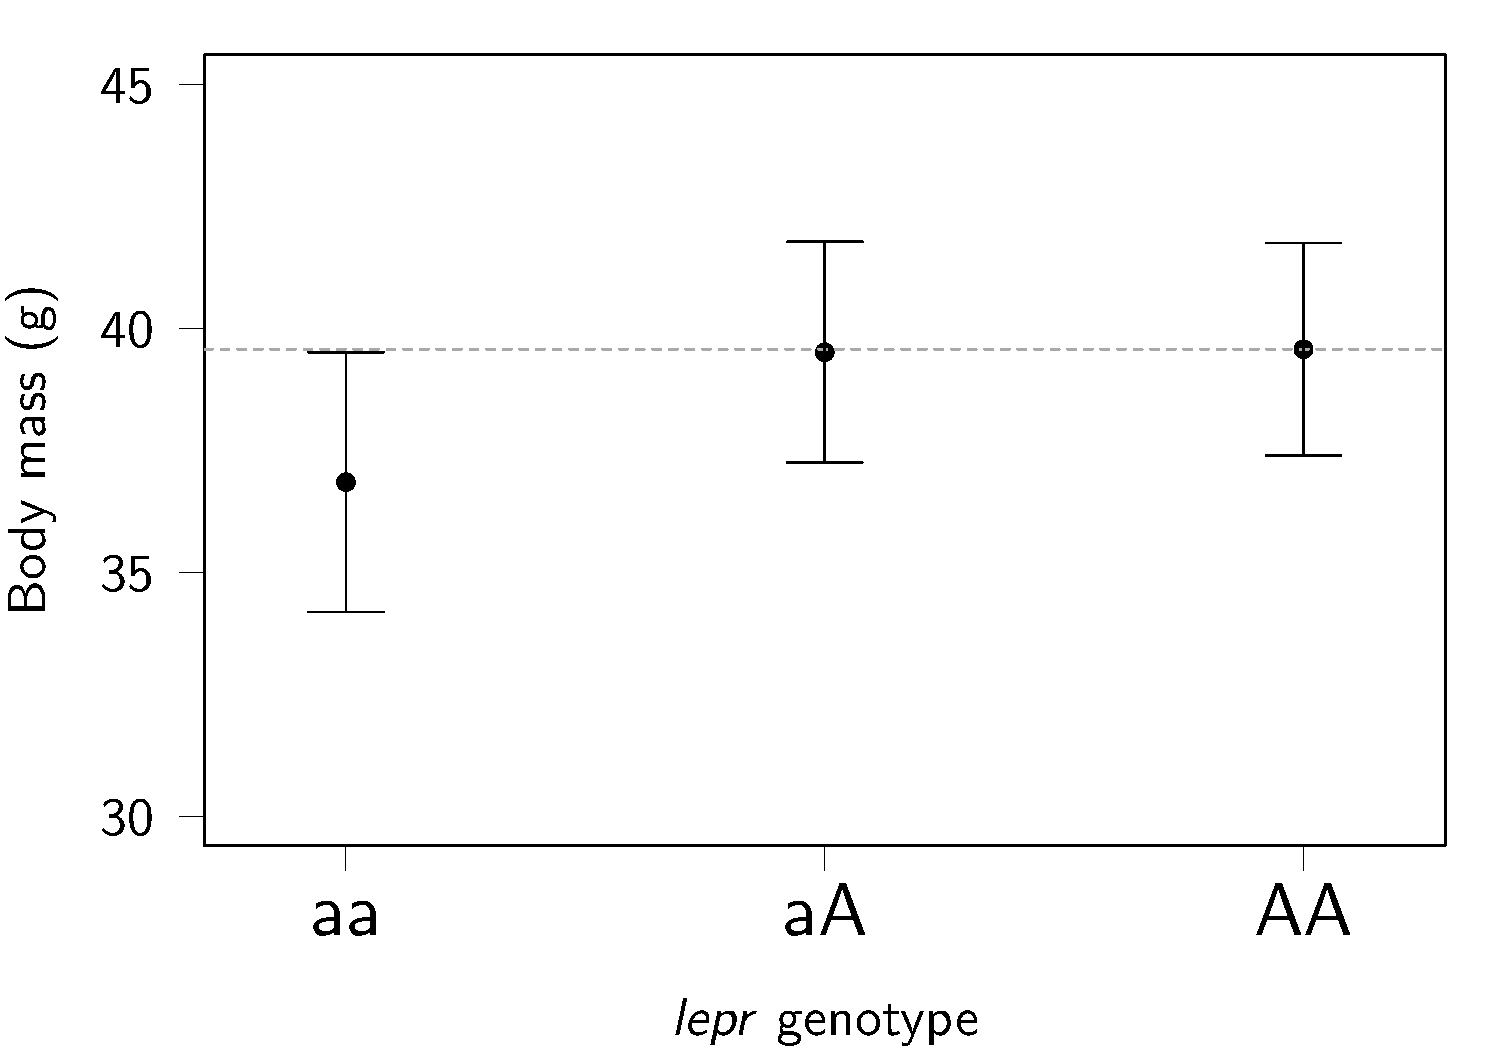
\includegraphics[width=\textwidth]{FiguresGeneral/PhenoEffect-1}
	\caption{}
	\label{fig:leprpheno}
\end{figure}

Despite such a dramatic effect, \emph{lepr} genotypic variation explains only 1.3\% of the additive genetic variation estimated from an animal model. in particular because the homozygotes \emph{aa} are rare (3\% of all individuals genotyped).

Could we not simply sequence many more genes to explain a larger proportion of genetic variation?
The uncertainty in the estimation of the effect of \emph{lepr} translates into a Bayesian p-value of $0.01$. 
If other genetic loci were analysed, 


%%%%%%%%%%%%%%%%%%%%%%%%%%%%%%%%%%%%%%%%%%%
\section{This thesis}

\subsection{Objectives}

\subsection{Churwalden snow voles}

\subsection{Thesis outline}


